\documentclass[11pt,a4paper,titlepage]{article}

%---------------------------------------------------------------
%---------------PACCHETTI---------------------------------------
\usepackage[utf8]{inputenc}	%latin1 per codifica del file ISO-8859-1
\usepackage{amsfonts}
\usepackage{graphicx}
\usepackage{amsmath}
\usepackage{amssymb}
\usepackage{amsthm}
\usepackage{leftidx} %left index carbonio 12 -> ${^{12}}C$
\usepackage{nicefrac} %1/2 -> \nicefrac{1}{2}
\usepackage{multirow}
\usepackage[margin=10pt, font=small, labelfont=bf]{caption}
\usepackage{subfig}
\usepackage{pdfpages}
\usepackage{xspace}
\usepackage{booktabs}
\usepackage{epstopdf}
\usepackage[export]{adjustbox}
\usepackage{dpfloat}
\usepackage{xspace}
\usepackage{verbatim}
%\usepackage{arydshln}
%\usepackage[a4paper,left=15mm,right=15mm, top=1cm, bottom=2cm]{geometry}
\usepackage{longtable}

%---------------------------------------------------------------
%---------------ALTRI COMANDI---------------------------------------
\graphicspath{{./images/}}
\hyphenation{}
\binoppenalty=10000 %impedisco alle formule matematiche in linea di essere spezzate
\relpenalty=10000 %impedisco alle formule matematiche in linea di essere spezzate
\setlength{\parindent}{0em} %impedisco identazione paragrafi

%---------------------------------------------------------------
%---------------COMANDI PERSONALIZZATI--------------------------
\newcommand{\fd}[2]{\frac{ \mathrm{d}{#1}}{ \mathrm{d}{#2}}}
\newcommand{\sd}[2]{\frac{ \mathrm{d}^2{#1}}{ \mathrm{d}{#2}^2}}
\newcommand{\fpd}[2]{\frac{ \partial{#1}}{ \partial{#2}}}
\newcommand{\spd}[2]{\frac{ \partial^2{#1}}{ \partial{#2}^2}}
%\newcommand{\diff}{\mathrm{d}}  %esiste il comando \dif
\newcommand{\virg}[1]{``{#1}''}
%\newcommand{\article}[6]{#1, \textit{#3} \textbf{#4}, #6 (#5).} %\articolo{autori}{titolo}{rivista}{numero riv.}{anno pubblicazione}{pagina/n°articolo} //\virgolette{\textit{#2}};
\newcommand{\ie}{\emph{i.e.}\xspace}
\newcommand{\eg}{\emph{e.g.}\xspace}
\newcommand{\DM}{Dark Matter\xspace}
\newcommand{\DE}{Dark Energy\xspace}
\newcommand{\DS}{Dark Sector\xspace}
\newcommand{\LCDM}{$\Lambda$CDM\xspace}
\newcommand{\abs}[1]{\lvert{#1}\rvert}
\newcommand{\Lagr}{\mathcal{L}}
\newcommand{\tr}{\mathrm{tr}}
\newcommand{\zinco}{\texttt{ZInCo}\xspace}
\newcommand{\gadget}{\texttt{Gadget-2}\xspace}
\newcommand{\ap}[1]{\textsuperscript{#1}}
\newcommand{\ped}[1]{\textsubscript{#1}}



\author{Enrico Garaldi}
\date{\today}
\title{\textbf{\Huge ZInCo} \\ a new code for zoomed cosmological Initial Conditions}

\begin{document}
\maketitle

\section{Introduction}
\zinco (\emph{\textbf{Z}oomed \textbf{In}itial \textbf{Co}nditions}) is a tool for manipulating initial conditions (ICs) suitable for cosmological numerical simulations with the N-body parallel code \gadget \cite{GADGET-2} \cite{GADGET}.\\
The code \zinco can perform three different manipulations of the ICs:
\begin{itemize}
\item \textbf{dilution}: the number of particles in the ICs is uniformly reduced and the particle properties are consequently updated;
\item \textbf{zoom}: a number of regions in a snapshot of a simulation are determined by the user and marked with different dilution values; the code follows the particles in this regions up to the ICs of the simulations and performs a differential dilutions in order to produce regions with different particle densities (i.e. different resolutions);
\item \textbf{cascade}: similar to the zoom procedure, but the number of regions (and sub-regions) can be specified by the user, while their positions are set randomly.
\end{itemize}

The code requires the user to specify the position and dimension of the resolution regions, along with their level of resolution, \ie how much the particles in a given region should be diluted. Thus, the possibility to set different levels of resolution allow smooth transitions between the high- and low- resolution regions. The complete list of the input parameters available is provided in Appendix \ref{Input_params}.

The \zinco code is among the first codes capable to process different particle types producing different levels of resolution for each of them. Although a number of different codes able to produce initial conditions with different levels of resolution are publicly available, it is unusual to find a multi-scale cosmological initial conditions code able to process different particle types. This unique feature of the code is due to the fact that, instead of producing multi-resolution initial conditions from scratch, the \zinco code uses already produced initial conditions. The latter can be produced featuring any particle types desired and require no further complication in the zooming procedure. 

Thus, the \zinco code provides both a simple and powerful tool for producing initial conditions which can be used for a large number of conceptually-different cosmological simulations

\section{Basic Structure of the code}
\label{Basic_struct}
The approach chosen for the code's development is to start with high-resolution ICs and then reduce the resolution where it is not needed. This approach, despite requiring more space for the storage of the initial realisation, ensures that in the region of interest (i.e. the high-resolution region), the particle positions are the same as in the high-resolution ICs. Moreover, this approach is somewhat backward compatible, since the code can process also already-existent ICs, whilst producing them from scratch would have meant that the existing simulations could not be processed.

The basic algorithm of the code divides the simulation box in cubic cells and produces new particles by summing or averaging the properties of the particles inside the same cell, depending on the resolution requested for the given cell. In such a way it is possible, starting from high-resolutions ICs, reduce their resolution when not needed and keeping it high in the regions of interest. The entire simulation box is divided in $CubesPerSide$ slices along each dimension, and thus the total number of cubic cells produced is $CubesPerSide^3$, where $CubesPerSide$ is a parameter which must be set as an input. The different resolution regions are ideally spherical regions, determined by the user or by the code (depending on the usage). However, since the dilution procedure is performed processing the simulation box one cubic cells at a time, the final shape is the one of a sphere made up of cubic pieces.

In order to describe how the selection of the resolution for a given cell is done, we start assuming a single resolution region. The code loops through all the cubic cells and for a given cell, it computes the distance between the cell center and the region center and compare it with the cell radius. In order to avoid the case when the cell center lies just outside the resolution region but a considerable portion of its volume lies inside, before comparing the two values as described, the code adds to the distance computed half the cubes diagonal. This ensures that no cells could be assigned to a lower resolution even if some of their volume cross a higher resolution regions. As a side effect, adding half the cube's diagonal could led to assign higher resolutions to cells that lie completely outside of the higher resolution region specified, depending on their spatial position. However, this side effect does not affect the region of interest (the high-resolution one) and on the contrary could \emph{extend} the high resolution region\footnote{This could lead to an increase in the final number of particles, and thus an increase in the computing resources needed. However, for typical values of the input parameters, this side effect only involve a negligible number of cells with respect to their total number.}.

In a more realistic case there are multiple resolution regions, possibly with different centres. In these cases, the procedure described above is repeated for every regions and the cells is assigned the highest resolution among the ones determined using the different regions. The number of resolution \emph{levels}, \ie the number of possible values for the resolution, can be set as an input parameter ($LevelsNumber$).

The code can process ICs which include different types of particles. Their number can be set through the parameter $SpeciesNumber$ and the different species must be stored in the first $SpeciesNumber$ slots, \ie their \gadget type must range from $0$ to $SpeciesNumber - 1$. Since \gadget can handle up to 6 particle species, and since each resolution region needs its own particles type, the following relation between the number of different resolution regions ($LevelsNumber$) and the number of particle species present in the ICs ($SpeciesNumber$) must hold true:
$$LevelsNumber * SpeciesNumber <= 6$$

Now we move to describe how the actual dilution of the ICs is performed. Once that every cell has been labelled with a given resolution level, the code performs a specific operation, depending on the input parameters given:
\begin{itemize}
\item \textbf{copy}: the particles inside the cell are copied in the new ICs;
\item \textbf{merge}: the particles inside one or more contiguous cells with the same resolution level are merged together, in order to produce a single particle in the new ICs (more details will follow);
\item \textbf{discard}: the particles inside the cell are ignored and thus they will not appear in the new ICs.
\end{itemize}

The first and the last operation are straightforward, but the second one is worth of a detailed discussion. The different dilution factor can be specified as a number of cubic cell to merge together. The cells are merged using cubic regions made of $Level<n>CubesPerSide$ (which is an input parameter) cells in every side, where $<n>$ is the level number and range from $0$ to $LevelsNumber - 1$. Clearly, the higher this number is, the lower the final resolution since a higher number of particles is merged. In the case the geometric distribution of the cells does not allow to have an adequate number of cubes to merge together, $Level<n>CubesPerSide$ is reduced by $1$ and the operation is repeated. In such a way it is ensured that all the cells with a given level of resolution are merged following as close as possible the input given.

When merging together a group of particles, the codes simply produces a new particles with:
\begin{itemize}
\item position and velocity which are the position and velocity of the center of mass of the particles of the group
\item mass which is the sum of the masses of the particles belonging to the group
\item a new unique ID
\end{itemize}

The newly produced particles are stored in a series of new ICs files, which the same format of the input ones. In particular, the first $SpeciesNumber$ types of particles correspond to the particles belonging to the higher level of resolution, the next $SpeciesNumber$ types correspond to the higher-but-one level of resolution, and so on.

\zinco has also the option to save in a file the correspondence between the old IDs (\ie the IDs of the particles in the original initial conditions) and the new IDs.

Since a common way of proceeding in cosmological zoomed simulations is to run first a simulation with low resolution in order to identify the regions to zoom in, the code provides a function called \virg{dilution} which uniformly reduces the resolution on the entire box. The differences between these two behaviours are shown in Figure \ref{Zoom_comparison}, where a slice of the initial conditions  box is shown: in the upper panel the original initial conditions are shown, in the middle one the result of their dilution is displayed, while in the bottom one the result of a zoom centred somewhere near the center of the box is plotted.

\zinco also provides the possibility to specify the different regions directly in a low-resolution output. The code will take care of tracing back the particles in the different regions to the low-resolution initial conditions, identifying the corresponding region in the high-resolution initial conditions and then produce the new zoomed ICs files.

\begin{figure}[!tb]
\centering
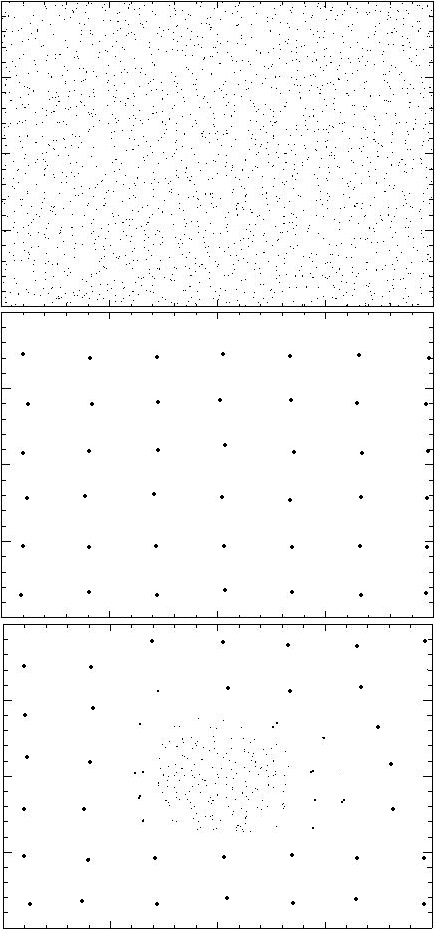
\includegraphics[height=0.4\textheight]{Zoom_comparison_tot.jpg}
\caption{Example of the zoom procedure: the first image shows a slice of the original high-resolution ICs, the second one shows the homogeneous dilution of the former and the third shows the different dilution in different zones centred in the box center.}
\label{Zoom_comparison}
\end{figure}


\section{Dilution}
The dilution is the simplest of the operations the code can accomplish and it consists in an uniform reduction of the resolution through the entire box. In this case the only important geometrical input parameter is $CubesPerSide$, since $LevelsNumber$ and $Level0CubesPerSide$ are both automatically set to $1$. This procedure is usually adopted in order to run a low-resolution simulation before the zoomed one using a set of ICs which is compatible with the zoomed one.

\section{Zoom}
The zoom procedure is thought in order to zoom in a single \virg{object} of interest. Thus, the resolution regions share the same center (ideally the center of the object one is interested in). Their radii are, however, set through input parameters.

The code requires three different list of particles in this case: the output of a simulation, which is the \virg{base} upon which the resolution regions are specified; the correspondent ICs; and the original ICs from which the former have been obtained. \zinco will check the particles belonging to the inner region in the output, storing their IDs. These will be used to trace back the particles to their initial conditions in order to update the radius of the inner region (the radii of the other regions will be update maintaining constant their ratio with the radius of the inner one) and the center (which is the same for every regions). Now, the procedure described in Section \ref{Basic_struct} is applied using the updated radii and center in order to produce the final ICs. An example of the procedure just described can be found in Figure \ref{Zoom_procedure}.

The radii of the resolutions regions are set through the input parameter $Level<n>BubbleRadius$ and the dilution parameter for the different levels through $Level<n>CubesPerSide$.

\begin{figure}[!p]
\centering
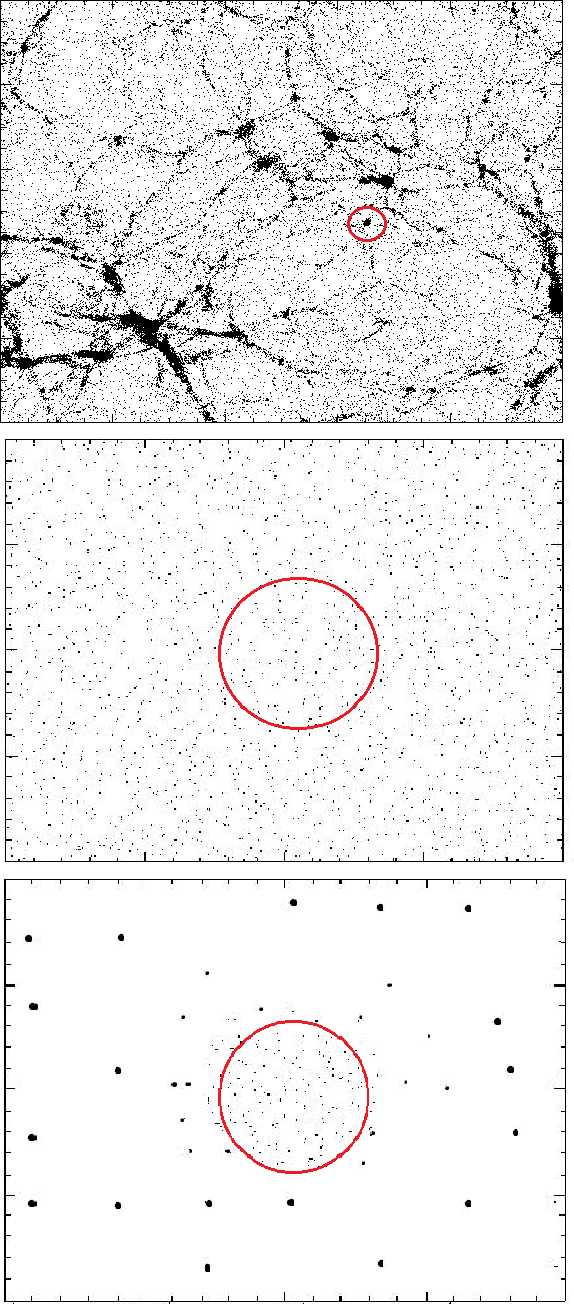
\includegraphics[height=0.4\textheight]{zoom_procedure_vert.png}
\caption{Example of the zoom procedure: the first image shows a slice of the snapshot at $z=0$ obtained from a simulation using diluted ICs; once a halo of interest is selected (red circle), its particles are traced back to its ICs and the high-resolution region selected is adapted (the second image). Then the code produces the three regions with different resolution around the halo selected in the new (zoomed) ICs (third image).}
\label{Zoom_procedure}
\end{figure}

\section{Cascade}
The cascade procedure is used to produce a simulation box which contains a certain number of spheres with higher resolution. This \virg{bubbles} contains other bubbles with higher resolution and so on. This is useful for producing large cosmological simulations which, however, allow to study in details some structures in a realistic cosmological potential, thanks to the bubbles of higher resolution.

The bubbles are created in random positions \emph{but} ensuring they are completely contained in a bubble of the previous level of resolution. In such a way, a smooth transition between low-resolution and high-resolution regions is ensured. Moreover, the bubbles of a given level does not intersect. The radii of these bubbles and the corresponding resolution are set in input. Note that if the $Level0$ bubble does not cover the entire simulation box, the particles outside the bubble will be discarded.

In this case, further input parameters are needed:
\begin{itemize}
\item \textbf{$Level<n>Size$} (for $<n>$ ranging from $0$ to $LevelsNumber - 1$) is used to set the number of Bubbles each level will contain;
\item \textbf{$CascadeRandomSeed$} which allows to set a random seed for the bubbles production.
\end{itemize}

\section{Tests of the code}
Here we present a series of test performed in order to ensure that the ICs produced by \zinco are suitable to be used in zoomed simulations. As a first test, we checked their power spectrum, which must be identical to the one of the original initial conditions, since they must represent the same statistical realisation with different resolution. In particular, the power spectra are expected to differ only at small scales, where the shot noise becomes relevant: less particles in the same box means a greater mean particles separation, resulting in a greater shot noise, that hence modifies the power spectra at slightly larger scales.

An initial set of $2 \times 512^3$ particles was produced and a series of dilutions was performed, obtaining different sets of initial conditions. Their power spectra were computed and the results are shown in Figure \ref{PowSp_compare}.

\begin{figure}[!tbp]
\centering
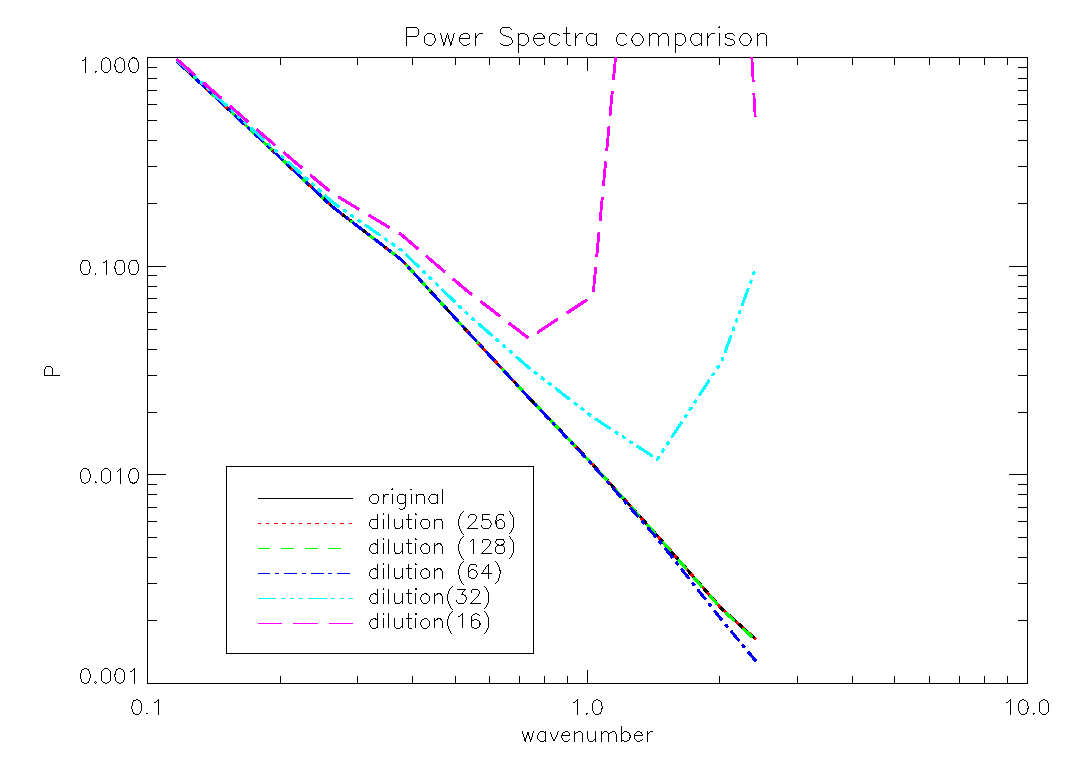
\includegraphics[width=\textwidth]{PowerSpectra_comparison.eps}
\caption{Comparison between the power spectrum of the original initial conditions and the ones obtained as different dilutions of the former. The original ICs contains $2 \times 512^3$ particles, while the dilutions contains $2 \times N^3$, where $N$ is the number written in parenthesis in the legend. As expected, they differ only at small scales, where the shot noise becomes relevant at different wavenumbers.}
\label{PowSp_compare}
\end{figure}

%The shot noise, which modifies the profiles at different scales, is due to the granularity of the particles, which becomes relevant at small scales, because the high momenta can't be reached due to the Nyquist limit. This type of noise modifies the power spectra adding a term
%\begin{equation}
%\langle \delta_{SHOT}\rangle = \frac{1}{N}
%\end{equation}
%where $N$ is the number of particles in the box. Hence, its dimensionless form is
%\begin{equation}
%\Delta^2_{SHOT} \propto \frac{1}{N} k^3
%\end{equation}
%This clearly shows that, as the number of particles decreases, the shot noise becomes more important. Hence, this term is different for the different dilutions of the ICs, while the non-noisy Power Spectra is the same, since the method used for the dilution preserves the original statistical realisation of the glass file, \ie the theoretical Power Spectrum of the initial conditions.

Since the power spectra obtained from the diluted initial conditions and the original ones are fully consistent, after taking into account the noise deviations, the results of the code described above can be trusted and, then, the new initial conditions can be used to perform a numerical simulation with modified resolution (diluted or zoomed).

Although the power spectra show that the code performs the dilution procedure in a consistent way, there is another test that must be made before using the zoomed initial conditions for a fully trustful numerical simulation: the high- and medium-resolution regions must be large enough to avoid the presence of \emph{intruders}, \ie particles of lower resolution which penetrate in the deeper part of a higher-resolution region, at low redshifts. This must be avoided since their presence could significantly perturb the gravitational dynamics of the high-resolution particles, resulting in modified and unrealistic results.

This check must be done separately for every zoomed simulation, since the minimum radius sufficient to avoid intruders is highly dependent on both the dimensions of the structure of interest and its evolution. An example of good and bad resolution regions choice is shown in Figure \ref{intruders}.

\begin{figure}[!tbp]
\begin{minipage}{0.5\textwidth}
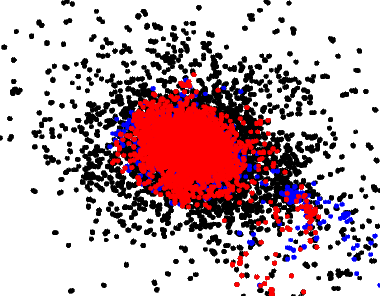
\includegraphics[width=\textwidth,left]{intruders1.png}
\end{minipage}
\begin{minipage}{0.5\textwidth}
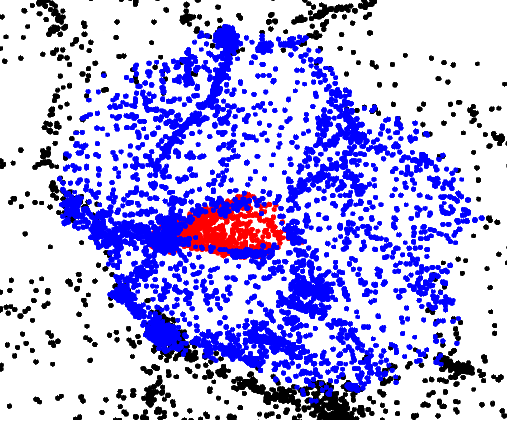
\includegraphics[width=0.95\textwidth,right]{intruders2.png}
\end{minipage}
\caption{The difference between a zoomed simulation with a too small (left panel) and a wide enough (right panel) mid-resolution region. The low-resolution particles are printed in black, the mid-resolution ones in blue and the high-resolution ones in red. In the left panel, the too small medium-resolution region is completely mixed with the high- and low-resolution ones. In the right picture, the regions are clearly separated, with the exception of the boundaries of the regions. The pictures are the $z=0$ snapshots of a simulation containing $2 \times 128^3$ particles with box side $80~Mpc/h$.}
\label{intruders}
\end{figure}

A final test consists in checking that the large scale structures in the simulation are not modified, since at large scales the \virg{fine structure}, \ie the fact that there is a heavy particle in place of a number of lighter particles, should not modify the results.

In Figure \ref{Dilution} is plotted the $z=0$ snapshot for two different simulations, the first one (printed with red dots) is a uniform dilution of a set of $2 \times 512^3$ particles down to $2 \times 128^3$ particles for each type, while the second (printed in blue) is a zoom around a single halo with a low-resolution equal to the diluted initial conditions, and double in the mid-resolution region. As one can clearly see, the large scale structure is the same for both the simulations, thus ensuring that the dilution procedure is faithful, since the red dots are hidden behind the blue ones, as a result of the almost perfect matching between the two simulation results.

\begin{figure}[!tbp]
\centering
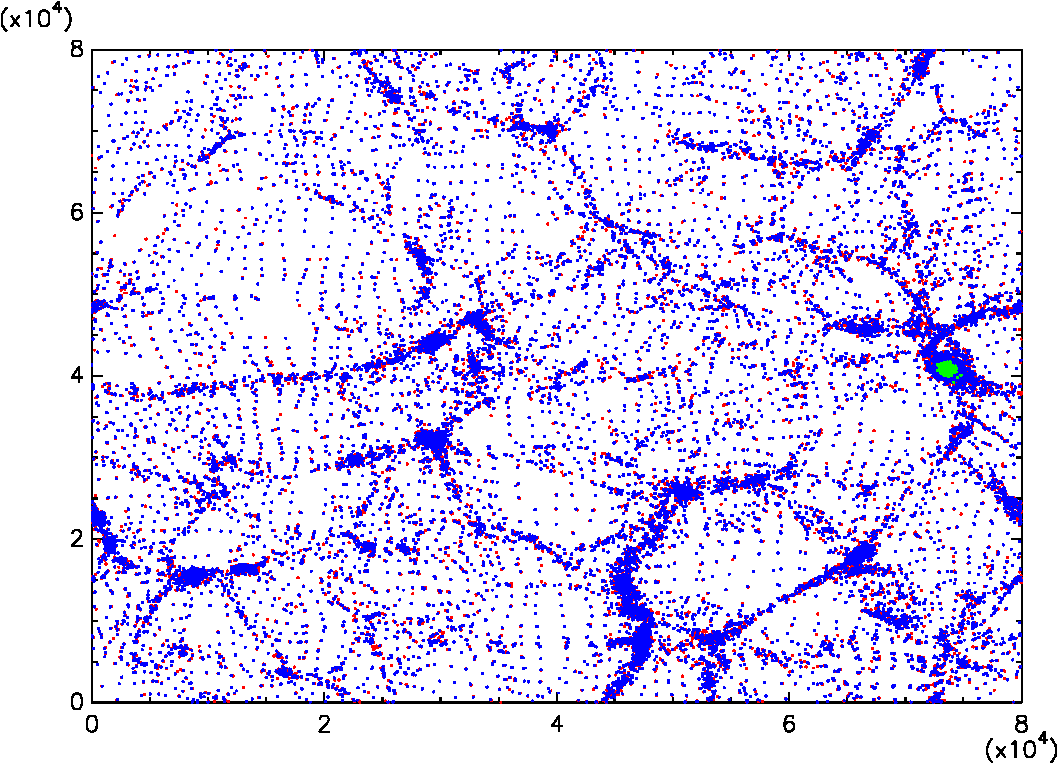
\includegraphics[width=\textwidth]{Slice_Dilute_vs_Zoom.pdf}
\caption{Snapshot at $z=0$ for initial conditions of $2 \times 512^3$ particles per type uniformly diluted to $2 \times 128^3$ particle per type (red dots) and for the same initial conditions zoomed around a single halo of interest with low resolution equal to the diluted one and medium resolution twice as many. In green are printed the particles of the zoomed halo. The simulation box has side $80~Mpc/h$, and the thickness of the slice is $1~Mpc/h$. The blue dots are plotted after the red ones, which thus are hidden behind them since they coincide almost everywhere. The axis report the position in unit of $kpc/h$, which are however not necessary for discussing the goodness of the zooming procedure.}
\label{Dilution}
\end{figure}

Besides testing the goodness of the produced zoomed initial conditions, some benchmark tests were also performed, in order to test how the time needed by the code varies when changing the input parameters. These tests are shown in Appendix \ref{ZInCo_app}.

\section{Bibliography}
\begin{thebibliography}{99}
\bibitem{GADGET-2}
Springel V., 2005, MNRAS, 364, 1105

\bibitem{GADGET}
Springel V., Yoshida N., White S. D. M., 2001, New Astronomy, 6, 51
\end{thebibliography}


\appendix
\section{Input Parameters}
\label{Input_params}
The input to the code are provided through a parameter file. In the following a description of each parameter is provided:

\begin{longtable}{l|l|c|c|c|p{4.3cm}}
\textbf{parameter name}    &  \textbf{type} & \textbf{D} & \textbf{Z} & \textbf{C} &  \textbf{description} \\
\hline
%Dilution                   &  int         & Y & Y & Y &  \makebox[4.3cm][s]{These three parameters} \\
%Zoom                       &  int         & Y & Y & Y &  \makebox[4.3cm][s]{are used to determine} \\
%Cascade                    &  int         & Y & Y & Y &  what kind of run must be executed. The code check that exactly one of the is equal to 1 while the others must be zero. \\
RunType                    &  string      & Y & Y & Y &  String which contains the type of run (dilution, zoom or cascade) \\
HighResICsDir              &  string      & Y & Y & Y &  Directory in which the high-resolution ICs are stored \\
HighResICsName             &  string      & Y & Y & Y &  Name of the file(s) containing the ICs \\
HighResICsFilesNumber      &  int         & Y & Y & Y &  Number of files containing the ICs \\
HighResICsFilesType        &  int         & Y & Y & Y &  Files type (1 or 2) \\
OutputDir                  &  string      & Y & Y & Y &  Directory in which the output are stored \\
OutputFilesNumber          &  int         & Y & Y & Y &  Number of files in the output ICs \\
OutputFilesType            &  int         & Y & Y & Y &  Files type (1 or 2) \\
CubesPerSide               &  int         & Y & Y & Y &  Number of cubic cells per side in which the simulations box is divided \\
LevelsNumber               &  int         & Y & Y & Y &  Number of resolution levels to produce \\
SpeciesNumber              &  int         & Y & Y & Y &  Number of species in the ICs. They must be stored in the high-resolution ICs provided as the first SpeciesNumber particles, i.e. from index 0 to index $SpeciesNumber-1$  N.B.: please note that the following relation must hold true: $LevelsNumber * $ $SpeciesNumber <= 6$ \\
Level0Size                 &  int         & N & N & Y & \makebox[4.3cm][s]{How many bubbles each} \\
Level1Size                 &  int         & N & N & Y & \makebox[4.3cm][s]{level will contain. Note} \\ 
Level2Size                 &  int         & N & N & Y & \makebox[4.3cm][s]{that in the case of a zoom,} \\ 
Level3Size                 &  int         & N & N & Y & \makebox[4.3cm][s]{this value will be} \\
Level4Size                 &  int         & N & N & Y & \makebox[4.3cm][s]{automatically set to 1.}\\
Level5Size                 &  int         & N & N & Y & Moreover, only the first $LevelsNumber$ values will be considered, the other will be ignored \\
Level0BubbleRadius         &  float       & N & Y & Y & \makebox[4.3cm][s]{This set the radius of} \\
Level1BubbleRadius         &  float       & N & Y & Y & \makebox[4.3cm][s]{the bubbles for each} \\
Level2BubbleRadius         &  float       & N & Y & Y & \makebox[4.3cm][s]{level of resolution. In} \\
Level3BubbleRadius         &  float       & N & Y & Y & \makebox[4.3cm][s]{the case of a zoom, the} \\
Level4BubbleRadius         &  float       & N & Y & Y & \makebox[4.3cm][s]{radius of the first one} \\
Level5BubbleRadius         &  float       & N & Y & Y & ($Level0$) will be adjusted in order to contain in the ICs all the particle it contains in the snapshot provided. The other radii are adjusted maintaining constant their ratio to the first one. Moreover, only the first $LevelsNumber$ values will be considered, the other will be ignored. The radii must decrease from $Level0$ to $Level<LevelsNumber-1>$ \\
Level0CubesPerSide         &  int         & N & Y & Y & \makebox[4.3cm][s]{This set the number of} \\
Level1CubesPerSide         &  int         & N & Y & Y & \makebox[4.3cm][s]{cubic cells that should be} \\
Level2CubesPerSide         &  int         & N & Y & Y & \makebox[4.3cm][s]{merged when creating the} \\
Level3CubesPerSide         &  int         & N & Y & Y & \makebox[4.3cm][s]{particles of the given level} \\
Level4CubesPerSide         &  int         & N & Y & Y & \makebox[4.3cm][s]{of resolution. Moreover,} \\
Level5CubesPerSide         &  int         & N & Y & Y & only the first LevelsNumber values will be considered, the other will be ignored. Use 0 to copy the particles as they are. Use -1 to ignore the particles. \\
LowResICsDir               &  string      & N & Y & N &  Directory in which the low-resolution (i.e. zoom snapshot) ICs are stored \\
LowResICsName              &  string      & N & Y & N &  Name of the file(s) containing the ICs \\
LowResICsFilesNumber       &  int         & N & Y & N &  Number of files containing the ICs \\
LowResICsFilesType         &  int         & Y & Y & Y &  Files type (1 or 2) \\
SnapshotDir                &  string      & N & Y & N &  Directory in which the snapshot is stored \\
SnapshotName               &  string      & N & Y & N &  Name of the file(s) containing the snapshot \\
SnapshotFilesNumber        &  int         & N & Y & N &  Number of files containing the snapshot \\
Snapshot  FilesType        &  int         & Y & Y & Y &  Files type (1 or 2) \\
x\_c                       &  float       & N & Y & N &  Coordinates of the center of the resolution regions \\
y\_c                       &  float       & N & Y & N & \\
z\_c                       &  float       & N & Y & N & \\
CascadeRandomSeed          &  int         & N & N & Y &  Random seed for the bubbles random production (if < 0 the seed is set using the current time)\\
CascadeMaxIter             &  int         & N & N & Y &  Maximum number of iteration done while trying to place a bubble\\

\hline

\end{longtable}

If you want to insert comments in the parameter file, you can do it by starting the comment with \%

\section{Compilation Options}
Here we describe the available compilation options.

\begin{longtable}{l|p{6cm}}
\textbf{option}                    &  \textbf{description} \\
\hline
DEBUG                              &  print informations about variables value during the whole run. It also performs a number of checks of consistency among the variables in key points of the code \\
VDEBUG                             &  Prints (a lot) of debug steps, approximately one for every group of related operation performed. Useful for determine the exact position where a problem occurs. \\
LONGIDS\_IN\_HIGH                  &  Use long IDs in the high-resolution ICs \\
LONGIDS\_IN\_LOW                   &  Use long IDs in the low-resolution ICs and in the snapshot \\
LONGIDS\_OUT                       &  Produce ICs with long IDs \\
VINFO                              &  Print a huge number of informations in the info.txt file. Be careful, the fill will become BIG! \\
PRINT\_IDS\_CORRESPONDENCE         &  Produce a file with the corrspondence between the IDs in the old (high-resolution) ICs and the new (processed) ICs \\
BARYONS                            &  Activate baryon treatment (i.e. reading and writing internal energies). Baryons \emph{must} be stored in type 0 in the original ICs. \\
\hline
\end{longtable}

\section{Output}
The code output consists in a series of file, all of them saved in the $OutputDir$ directory:
\begin{itemize}
\item $OutputFilesNumber$ file(s) containing the processed ICs. They have the same name as the high-resolution ICs files but appended with \virg{.dilution$<CubesPerSide$>}, \virg{.zoom} or \virg{.cascade} for the three different procedure available;
\item info.txt, containing informations about the code operations and timing;
\item [optional] ID\_correspondece.txt, which contains the correspondence between the initial IDs of the particles and the new ID, i.e. the ID they have in the new ICs produced.
\end{itemize}

Moreover, some informations are printed on screen during the run. They are mainly related to the file processed and the subroutine running. A copy of the parameter files used is saved in the same directory as the original parameter file and with the same name but appended with \virg{-usedvalues}.

\section{Benchmark}
In this Section the results of a small series of benchmark tests of the \zinco code will be described.

The code has been tested performing a series of clocked dilutions in different situations. In particular, the differences were in
\begin{itemize}
\item the initial conditions: the code was run with a series of initial conditions which differ each other both for the number of particles contained in the box and the number of files they are made of. The majority of the tests were performed diluting initial conditions containing $2 \times 256^3$ or $2 \times 512^3$ particles per type, both of them spread upon 8 files, but a smaller number of test runs were made using initial conditions containing $2 \times 1024^3$ particles per type;
\item the dilution factor: the dilution factor used are \virg{2x}, \virg{4x}, \virg{8x}, \virg{16x}. A dilution factor of \eg \virg{2x} means that the final number of particles one eighth (\ie $1/2^3$) of the initial one. Thus, the grater the dilution factor, the smaller the final number of particles;
\item the number of used processors: the tests were made using 2, 4, or 12 processors
\end{itemize}
Every other parameter was kept fixed, including the memory-per-processor and, obviously, the supercomputing cluster used.

In Figure \ref{benchmark_wtaVSnp} is shown the wall-clock time (\ie the real time elapsed between the start and the end of the run) used for a dilution of $2 \times 256^3$ (left panel) and $2 \times 512^3$ particles (right panel) using different numbers of processors and different dilution factors (the different colors in the plots). The plot clearly shows that the time needed by the code is substantially independent of the dilution factor. This feature is not unexpected, since the code has to read each particle independently by the final number of diluted particles. The only difference is in the number of average operations (\ie the computation of the center of mass of a group of particles). Since they are much faster with respect to the reading of the particles from the initial conditions files, the elapsed wall-clock time is essentially independent of the dilution factor.

\begin{figure}[!tb]
\begin{minipage}{0.45\textwidth}
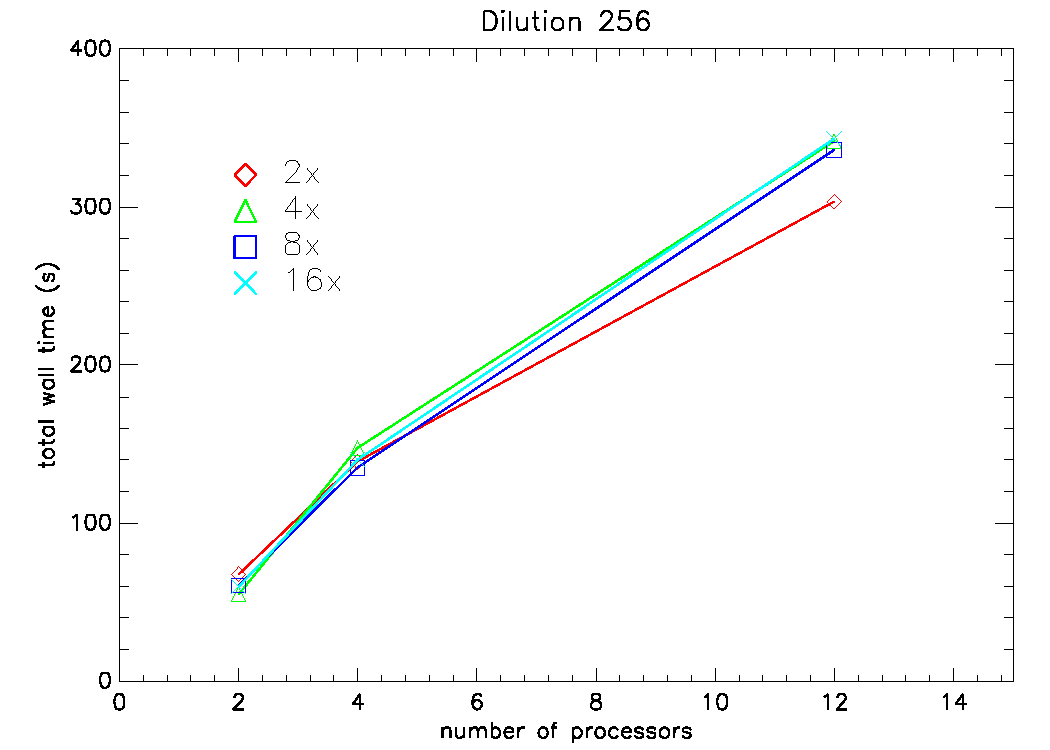
\includegraphics[width=\textwidth]{benchmark_wtaVSnp_256.pdf}
\end{minipage}
\begin{minipage}{0.45\textwidth}
\begin{flushright}
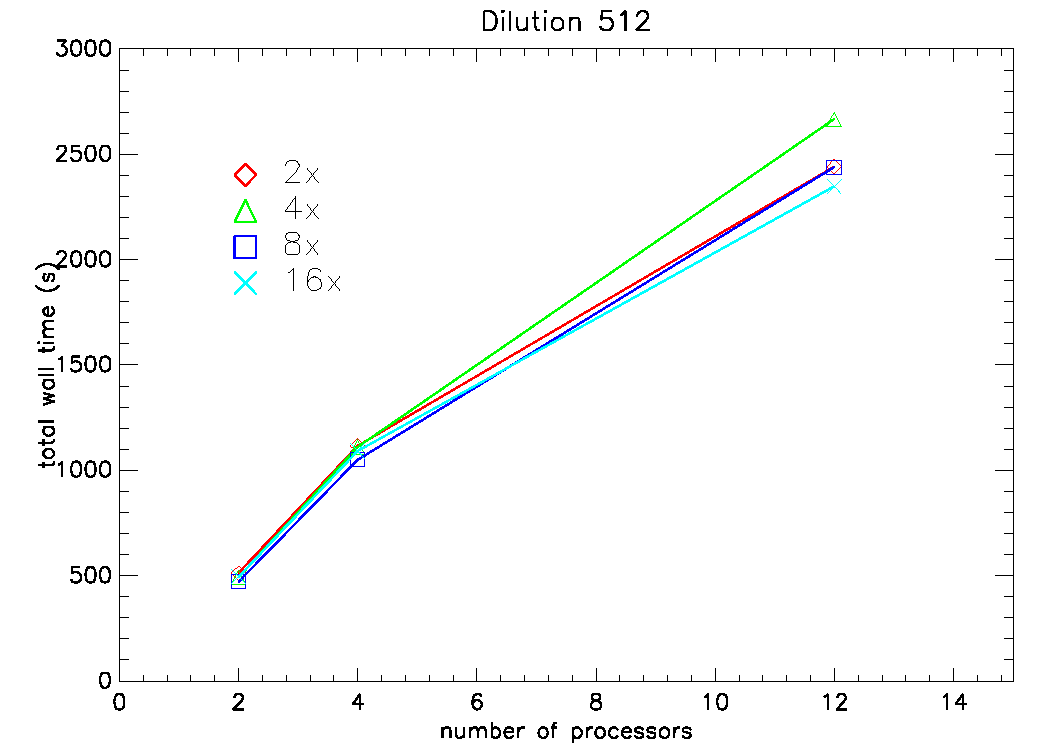
\includegraphics[width=\textwidth]{benchmark_wtaVSnp_512.pdf}
\end{flushright}
\end{minipage}
\caption{Wall-time used by different runs of the \zinco code for two different sets of initial conditions: the ones relative to the left-hand-side panel contain $2 \times 256^3$ particles, whilst the ones on the right-hand-side panel contain $2 \times 512^3$ particles.}
\label{benchmark_wtaVSnp}
\end{figure}

For the same reason, \ie the predominance of the time necessary to the reading of the particles from the file they are written in with respect to the time required by the arithmetical operations performed by the code, there is a large increase of the elapsed time when passing from the initial conditions with $2 \times 256^3$ particles to the one with $2 \times 512^3$ particles.

At a first glance, it could result surprising that the code does not improve its performances increasing the number of cores but, on the contrary, the elapsed wall-clock time increases for larger number of cores. This is due to the time necessary for the communication between the different processes, which  obviously increases as the involved processors increase in number. Thus, the number of processor used should be as small as possible. However, the code has been written in a parallel way since there are cases in which the processors number must be increased. This typically happens when the memory-per-processor is low, or vice versa when the diluted initial conditions contain a high number of particles, and in turn also the original ones do. In the latter cases, the parallelization allows to lower the memory requested by each processor since each of them has to store a smaller number of diluted particles (only the ones relative to the portion of simulation box assigned to it).

A further factor which modifies the time needed by the code is the dislocation of the processors. Typically the processors within the same core of the supercomputing cluster are equipped with a much faster interconnection with respect to the interconnection between different cores. Thus, if the processors used are located in different cores, the measured wall-clock time becomes much greater. Thus, the almost linear growth shown in Figure \ref{benchmark_wtaVSnp} is bound to become non-linear as soon as the number of used processors exceeds the number of processors within a single node.

This effect can be qualitatively evaluated running the code on the $2 \times 256^3$ particles' initial conditions with two processors located in the same core (named \virg{2 cores}) or in different cores (named \virg{1+1 cores}) of the PLX cluster. The results are shown in Table \ref{benchmark_2VS1+1}, where a significant increase (more than 30\%) in the elapsed wall-clock time is found.

\begin{table}[!h]
\centering
\begin{tabular}{r|c}
          &    elapsed wall-clock time (s) \\
\hline
2 cores   &    63.89 \\
1+1 cores &    83.53  \\
\end{tabular}
\caption{Comparison between the performances of the \zinco code run with two processors in the same core (named \virg{2 cores}) or in different cores (named \virg{1+1 cores}).}
\label{benchmark_2VS1+1}
\end{table}

As stated earlier, a small number of runs using initial conditions with $2 \times 1024^3$ particles were performed. Although not extensive as the ones described above, the results uphold the trends and conclusions obtained for smaller initial conditions. The results available for these larger initial conditions are reported in Table \ref{Tab_1024}. They show that the wall-clock time is in fact independent of the dilution factor (a dilution factor of 2x or 8x produce a difference in the elapsed time smaller than 16\%), whilst it is almost linearly increasing with the number of used processors.

\begin{table}[!h]
\centering
\begin{tabular}{cc|c}
np & dil                  & elapsed wall-clock time (s) \\
\hline
2  & 2x  & 4722.79 \\
4  & 2x  & 9504.46 \\
2  & 8x  & 3975.27 \\
\end{tabular}
\caption{The available benchmark results for the $2 \times 1024^3$ particles initial conditions. \virg{np} is the number of processors used and \virg{dil} is the dilution factor.}
\label{Tab_1024}
\end{table}

Turning to analyse the dependence of the wall-clock time elapsed on the dilution factor used in the simulation, \ie keeping fixed the number of used processors, it turns out that it is almost independent of the dilution factor, as shown in Figure \ref{benchmark_wtaVSdil}. This conclusion match with the observation that the code must read all the particles in every case, and since this is the most time-consuming operation, the elapsed time is almost constant as long as the same set of initial conditions is used.

\begin{figure}[!tb]
\begin{minipage}{0.45\textwidth}
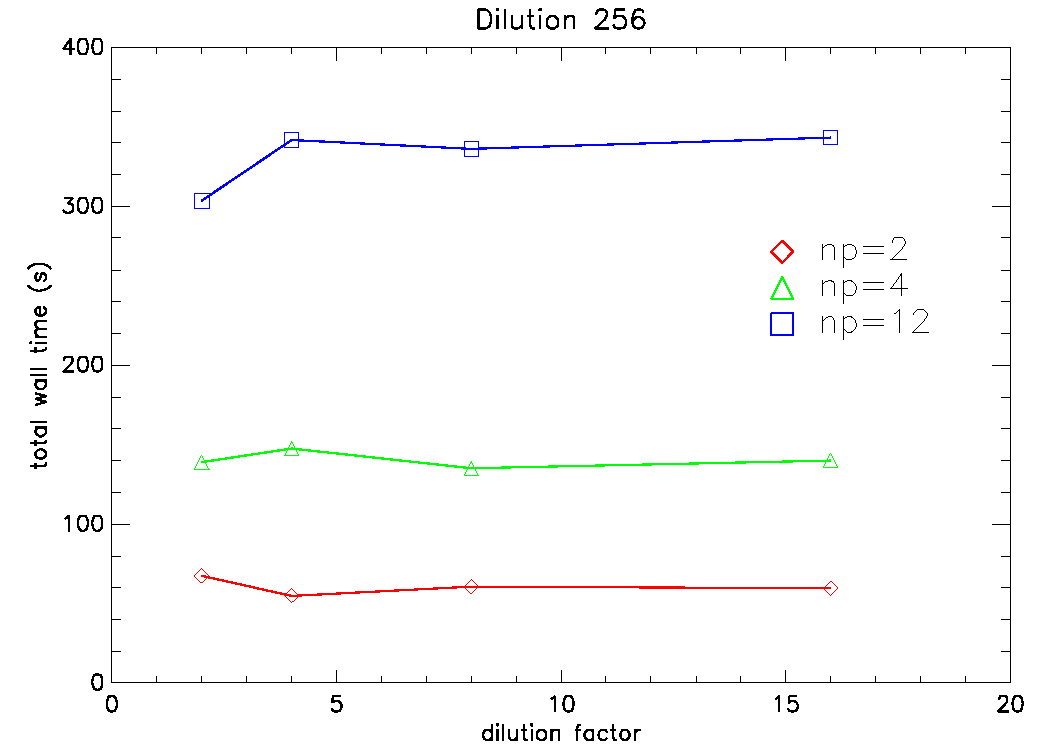
\includegraphics[width=\textwidth]{benchmark_wtaVSdil_256.pdf}
\end{minipage}
\begin{minipage}{0.45\textwidth}
\begin{flushright}
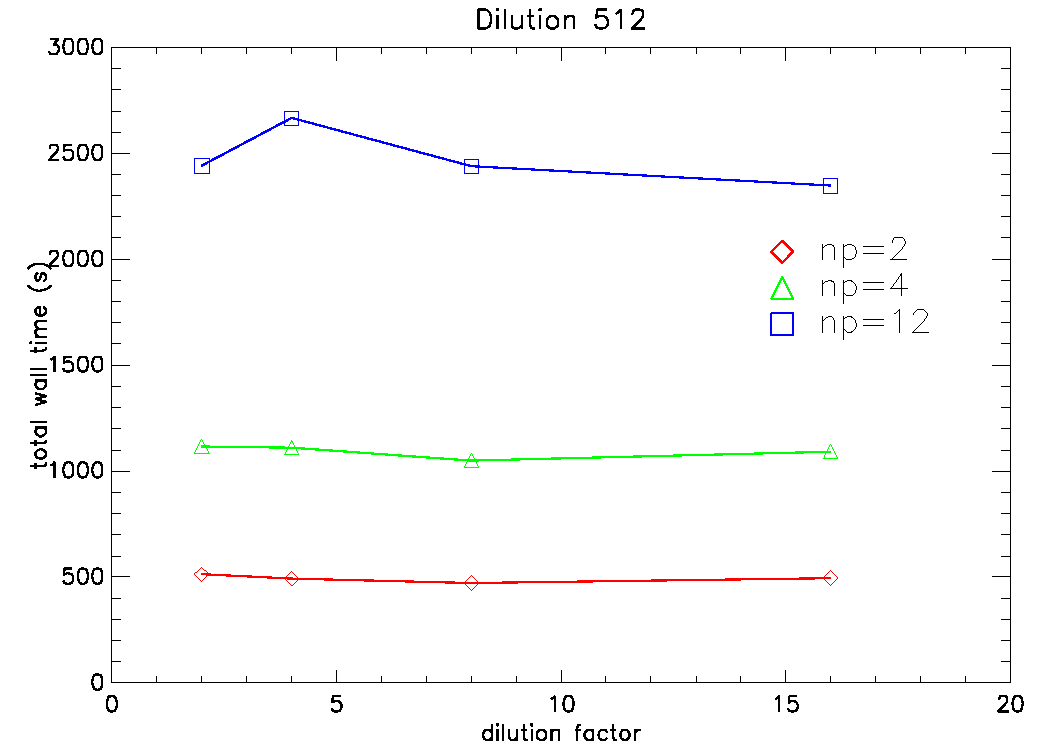
\includegraphics[width=\textwidth]{benchmark_wtaVSdil_512.pdf}
\end{flushright}
\end{minipage}
\caption{Wall-time used by different run of the \zinco code for two different sets of initial conditions: the ones relative to the left-hand-side contains $2 \times 256^3$ particles, whilst the one on the right-hand-side contains $2 \times 512^3$ particles. The different sets of points (each one of them denoted by a different colour) refer to different series of run using different number of processors ($np$).}
\label{benchmark_wtaVSdil}
\end{figure}

The tests described were performed diluting the initial conditions to different final states. However, no significant differences in the performances are expected between the dilution or zooming procedure, with the exception of an increase in the elapsed time independent of the number of processors and roughly proportional to the number of particles present in the initial conditions. These effects are results of two different portions of the code: in the core, where the dilution or zoom take place, no differences are expected since the only difference is that in the first case the code averages over a certain number of particles while in the last case it simply copies the read particles. This operation, however, is much faster than the reading of the initial conditions (as shown before) and thus do not significantly modify the code performance. The real difference is that in the case of a zoom the code must firstly read the snapshot file, identify the regions of different resolutions, trace back the particles to the initial conditions and then compute the new regions of high- and medium-resolution, while in the dilution case all these operations can be avoided, since there is no difference between the particles. Thus, the time employed for these preliminary operations increases the total wall-clock time. For the reasons described above, the added time is substantially independent of the dilution factor. Moreover, since the code performs such computations in a serial way (only one processor does the effective computation and then transmits the results to the other processors), it does not depend on the number of employed processors. However, as the number of particles increases, also the time required for them to be read increases, introducing a dependence on the initial conditions' size.

These conclusions are supported by the benchmark curves obtained for the zoom procedure (instead of the dilution) which are shown in Figures \ref{benchmark_wtaVSnp_zoom} and \ref{benchmark_wtaVSdil_zoom} which are similar to the ones discussed above for the dilution procedure.

\begin{figure}[!tb]
\begin{minipage}{0.45\textwidth}
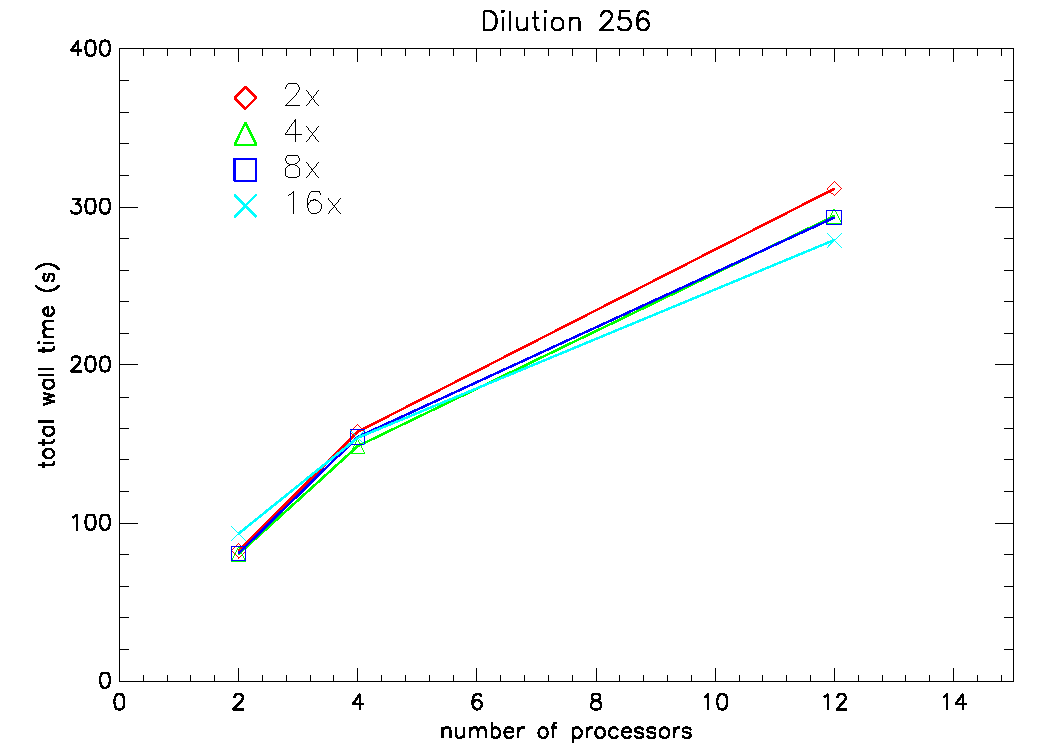
\includegraphics[width=\textwidth]{benchmark_wtaVSnp_256_zoom.pdf}
\end{minipage}
\begin{minipage}{0.45\textwidth}
\begin{flushright}
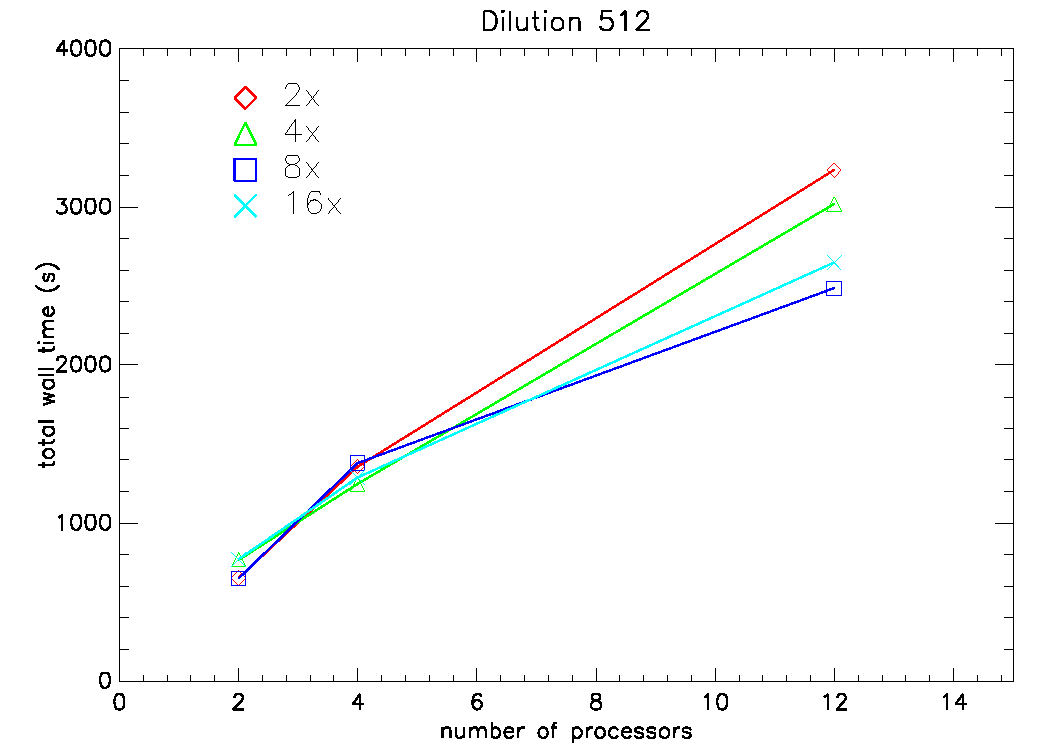
\includegraphics[width=\textwidth]{benchmark_wtaVSnp_512_zoom.pdf}
\end{flushright}
\end{minipage}
\caption{Wall-time used by different run of the \zinco code for two different sets of initial conditions: the ones relative to the left-hand-side contains $2 \times 256^3$ particles, whilst the one on the right-hand-side contains $2 \times 512^3$ particles.}
\label{benchmark_wtaVSnp_zoom}
\end{figure}

\begin{figure}[!tb]
\begin{minipage}{0.45\textwidth}
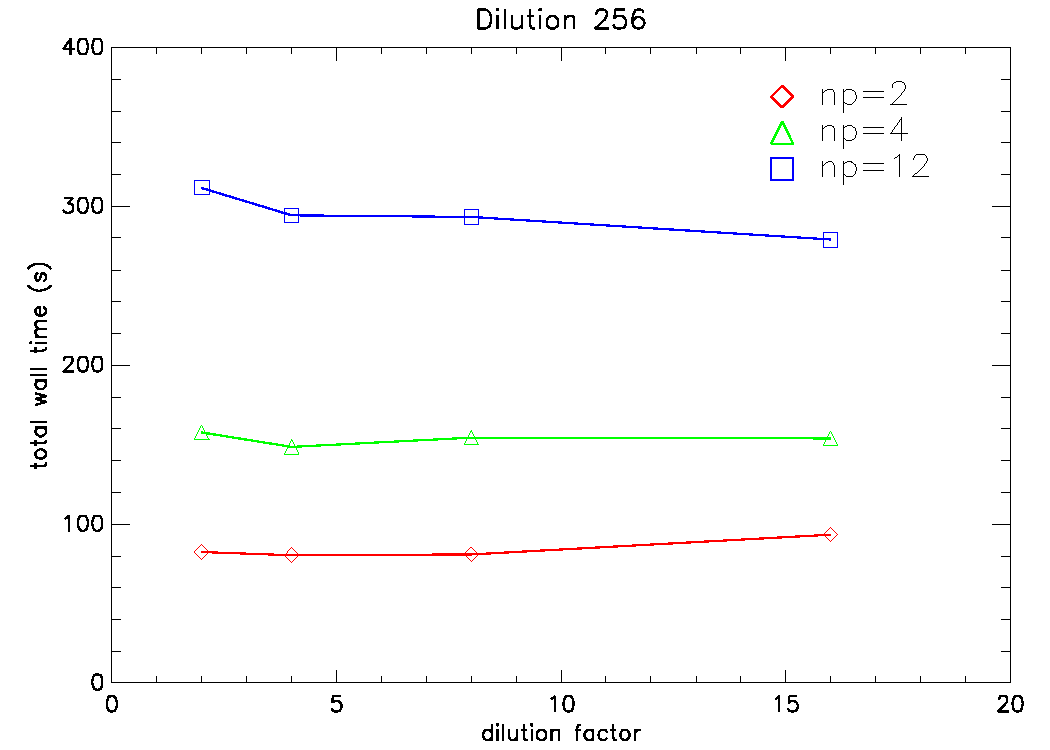
\includegraphics[width=\textwidth]{benchmark_wtaVSdil_256_zoom.pdf}
\end{minipage}
\begin{minipage}{0.45\textwidth}
\begin{flushright}
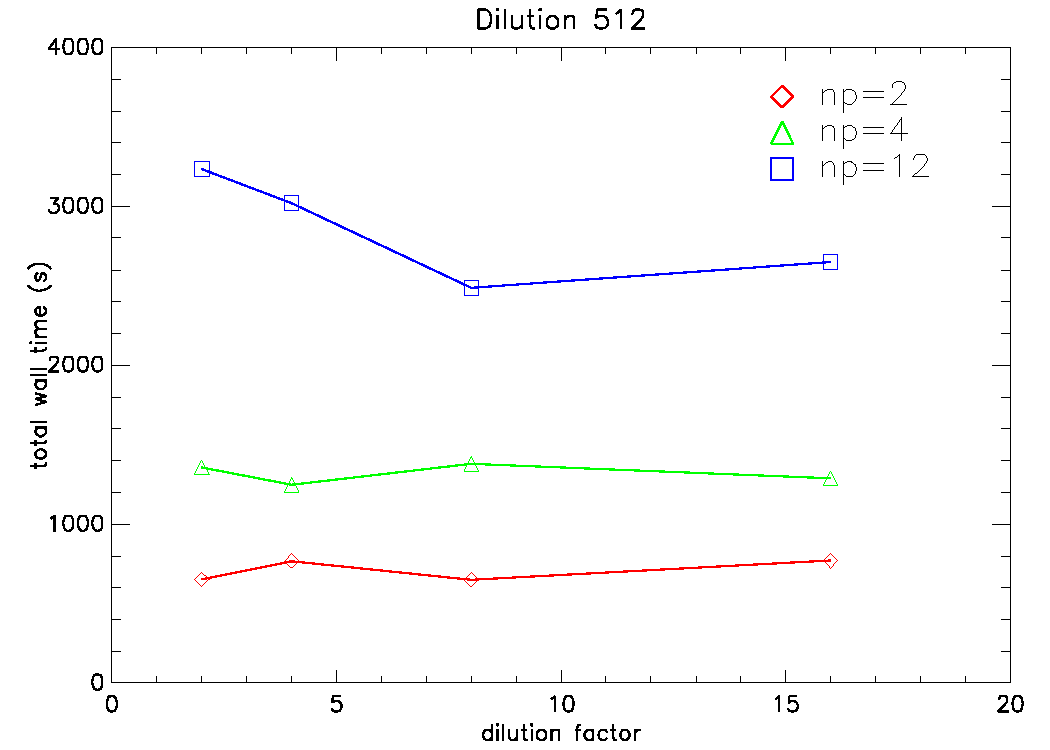
\includegraphics[width=\textwidth]{benchmark_wtaVSdil_512_zoom.pdf}
\end{flushright}
\end{minipage}
\caption{Wall-time used by different run of the \zinco code for two different sets of initial conditions: the ones relative to the left-hand-side contains $2 \times 256^3$ particles, whilst the one on the right-hand-side contains $2 \times 512^3$ particles. The different sets of points (each one of them denoted by a different colour) refer to different series of run using different dilution factors.}
\label{benchmark_wtaVSdil_zoom}
\end{figure}

Moreover, in Figure \ref{benchmark_regions} we plot only the time employed by the code for the computation of the new high- and medium-resolution regions. It is almost constant for different combinations of number of processors and dilution factors (in the Figure labelled on the x-axis as \virg{run}), as expected, and varies only as a function of the initial conditions, since the number of particles to be read changes.

\begin{figure}[!tbp]
\centering
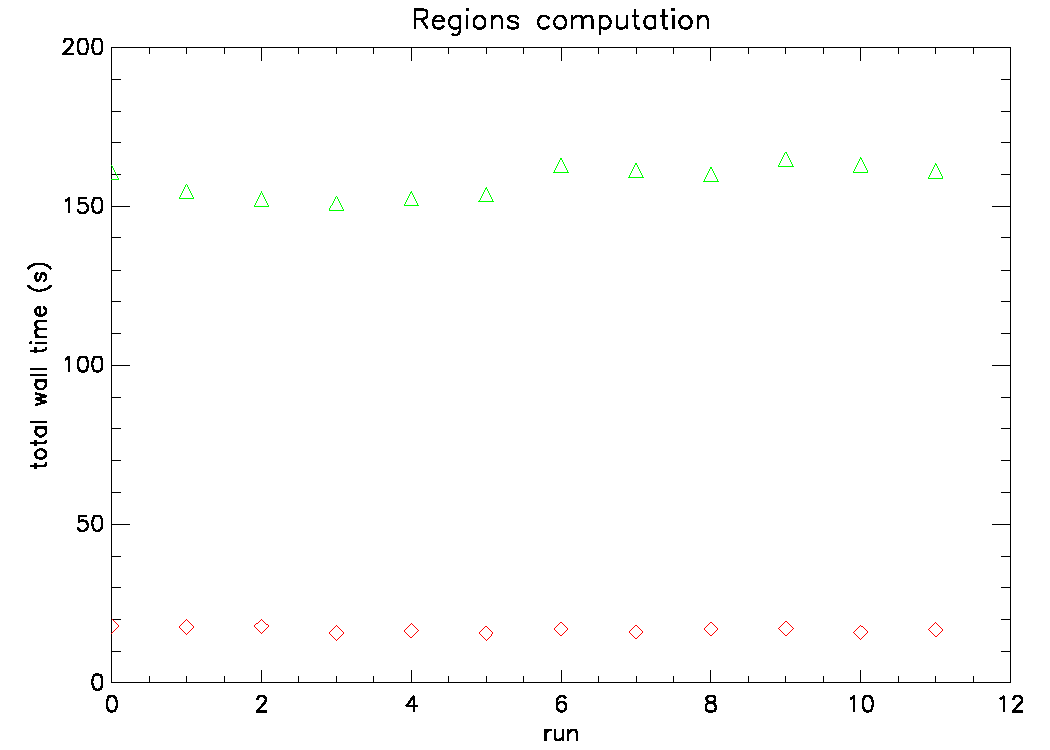
\includegraphics[width=\textwidth]{benchmark_regions.pdf}
\caption{Wall-clock time employed by the code to compute the new high- and medium-resolution regions for different numbers of processors, dilution factors and initial conditions. The label \virg{run} represents all the possible different combinations of number of processors (2,4,12) and dilution factor (2x, 4x, 8x, 16x).}
\label{benchmark_regions}
\end{figure}


Finally, in the previous tests the code read the the input files (\ie the initial conditions only, since they all refers to dilutions) with a serial algorithm. In the code it is also possible to perform the reading of the files using a parallel algorithm. However, this results in a very high increase in the wall-clock time employed by the code, as shown in Table \ref{parallel_vs_serial} where the results for dilutions using different numbers of processors are presented (here, as in Table \ref{benchmark_2VS1+1}, \virg{1+1} means two processors located in different cores of the supercomputing cluster) both in the case of serial and parallel reading. In all the cases presented the parallel reading needs more than 45\% the time needed by the serial reading. Since the difference in these two cases is just the parallel or serial nature of the algorithm used in reading the files, there are no reasons why this trend should be modified for different initial conditions or dilution factors.

\begin{table}[!h]
\centering
\begin{tabular}{cc|c|c}
    &     & \multicolumn{2}{c}{wall-clock time elapsed (s)} \\
np  & dil & parallel     & serial \\
\hline
2	& 2	  & 3195.10  & 67.59 \\
1+1	& 2	  & 4649.62  & 83.53 \\
4	& 2	  & 4750.41  & 138.83 \\
\end{tabular}
\caption{The available benchmark results for the $2 \times 256^3$ particles initial conditions read using both serial and parallel algorithm. \virg{np} is the number of processors used and \virg{dil} is the dilution factor.}
\label{parallel_vs_serial}
\end{table}


\end{document}
